\chapter{Introduction to Recurrent Neural Networks}
	\section{What is a Recurrent Neural Network?}
	
	\begin{itemize}
		\item Recurrent neural networks or RNNs (Rumelhart et al.,1986a) are a family of
		neural networks for processing sequential data.
		\item  Much as a convolutional network is a neural network that is specialized for processing a grid of values X such as an image, a recurrent neural network is a neural network that is specialized for
		processing a sequence of values $\{x^{(1)}, . . . , x^{(\tau)}\}$.
		\item Most recurrent networks can also process sequences of \textbf{variable} length.
	\end{itemize}
	
	\subsection{Motivation of RNN}
		\textbf{Parameter sharing!} \\
		Reasons why we need parameter sharing:
		\begin{itemize}
			\item  Parameter sharing makes it possible to extend and apply the model to examples of different forms
			(or different lengths) and generalize across them.
			\item  If we had separate parameters for each value of the time index, we could not generalize to sequence lengths not seen during training, nor share statistical strength across different sequence lengths
			and across different positions in time. 
		\end{itemize}
	
		\textbf{How to use the parameter sharing?}
		\begin{itemize}
			\item In the Recurrent networks, each member of the
			output is a function of the previous members of the output.	
			\item Each member of the output is produced using \textbf{the same update rule} applied to the previous outputs. This recurrent formulation results in the sharing of parameters through a very deep computational graph.
		\end{itemize}

	\subsection{Vanilla RNN}
	\begin{itemize}
		\item 
		\textbf{Training Data of the model} \\
		Here we use the sentence generation as the model, which aims to predict the next character in a sentence given all the characters before. \\
		 In this model, each $\mathbf{x}_i^{(t)}$ is a character in the sentence(represented as a $0-1$ vector), and the target is the next character which is also represented as a $0-1$ vector.
		\item
		\textbf{The structure of the network} \\
		It's an example of a recurrent network that maps an
		input sequence to an output sequence of the same length. \\
		The input of the network is $\{\mathbf{x}_i^{(1)},\mathbf{x}_i^{(2)},\dots,\mathbf{x}_i^{(\tau)}\}_{i=1}^N$, where N is the number of the samples, $\tau$ is the length of each input, and each $\mathbf{x}_i^{(t)}$ is a vector in the vector space $\mathbb{R}^n$. \\
		 The output is $\{\mathbf{y}_i^{(1)},\mathbf{y}_i^{(2)},\dots,\mathbf{y}_i^{(\tau)}\}_{i=1}^N$, the meaning of N and $\tau$ is the same, while each $\mathbf{y}_i^{(t)}$ is a vector in the vector space $\mathbb{R}^m$. \\
		\begin{figure}[H]
			\centering
			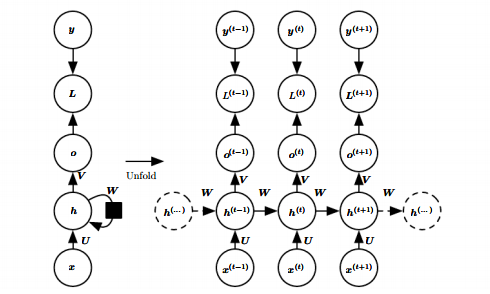
\includegraphics[width=0.9\textwidth]{VaRNN}
			\caption{The structure of Vanilla RNN}
		\end{figure}
		
		\item
		\textbf{The update equations for the forward propagation} is
		\begin{flalign*}
		\mathbf{a}^{(t)} &= \mathbf{b} + \mathbf{Wh}^{(t-1)} + \mathbf{Ux}^{(t)} \\
		\mathbf{h}^{(t)} &= tanh(\mathbf{a}^{(t)}) \\
		\mathbf{O}^{(t)} &= \mathbf{c} + \mathbf{Vh}^{(t)} \\
		\hat{\mathbf{y}}^{(t)} &= softmax(\mathbf{O}^{(t)})
		\end{flalign*}
		where the parameters are bias vectors $\mathbf{b}$ and $\mathbf{c}$ along with the weight matrices
		$\mathbf{U}$, $\mathbf{V}$ and $\mathbf{W}$, respectively for input-to-hidden, hidden-to-output and hidden-to- hidden connections.

		\item
		\textbf{The computation of the loss} \\
		For a given sequence of $\mathbf{x}$ values paired with a sequence of $\mathbf{y}$ values, the total loss would then be just the sum of the losses over all the time steps.\\
		For example, if $L^{(t)}$ is the negative log-likelihood of $y^{t}$ given $\{\mathbf{x}^{(1)},\ldots,\mathbf{x}^{(t)} \}$, the total loss is
		\begin{flalign*}
		L({\mathbf{x}^{(1)},\ldots,\mathbf{x}^{(\tau)}},{\mathbf{y}^{(1)},\ldots,\mathbf{y}^{(\tau)}}) \\
		= \sum_{t=1}^{\tau} L^{(t)}  \\
		= - \sum_{t=1}^{\tau} log p_{model}(\mathbf{y}^{(t)} |{\mathbf{x}^{(1)},\ldots,\mathbf{x}^{(t)}}) 
		\end{flalign*}
		where $p_{model}(\mathbf{y}^{(t)} |{\mathbf{x}^{(1)},\ldots,\mathbf{x}^{(t)}}) $ is given by the following rule:\\
		Denote the $\mathbb{R}^m$ output vector $\hat{\mathbf{y}}^{t}$ as $(\hat{y}_1^{(t)},\hat{y}_2^{(t)},\dots,\hat{y}_m^{(t)})$,and the target vector (a $0-1$ vector) is $(y_1^{(t)},y_2^{(t)},\dots,y_m^{(t)})$ while $y_i^{(t)} = 1$ and all the other elements of the vector is 0. Then 
		\begin{equation}
		p_{model}(\mathbf{y}^{(t)} |{\mathbf{x}^{(1)},\ldots,\mathbf{x}^{(t)}}) = \hat{y}_i^{(t)}
		\end{equation}
	\end{itemize}

	\subsection{Some important design patterns for RNN}
		\begin{itemize}
			\item Recurrent networks that produce an output at each time step and have recurrent connections only from the output at one time step to the hidden units at the next time step.
			\begin{figure}[H]
				\centering
				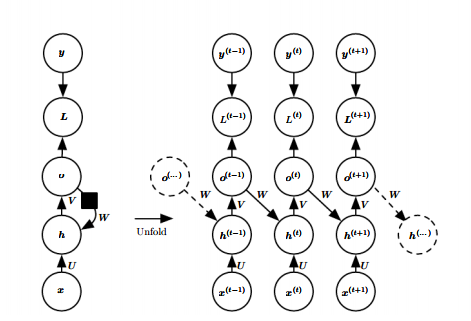
\includegraphics[width=0.9\textwidth]{O2HRNN}
				\caption{The structure of RNN(Output to Hidden)}
			\end{figure}
			\textbf{The update equations for the forward propagation} is
			\begin{flalign*}
			\mathbf{a}^{(t)} &= \mathbf{b} + \mathbf{WO}^{(t-1)} + \mathbf{Ux}^{(t)} \\
			\mathbf{h}^{(t)} &= tanh(\mathbf{a}^{(t)}) \\
			\mathbf{O}^{(t)} &= \mathbf{c} + \mathbf{Vh}^{(t)} \\
			\hat{\mathbf{y}}^{(t)} &= softmax(\mathbf{O}^{(t)})
			\end{flalign*}
			where the parameters are  bias vectors $\mathbf{b}$ and $\mathbf{c}$ along with the weight matrices
			$\mathbf{U}$, $\mathbf{V}$ and $\mathbf{W}$, respectively for input-to-hidden, hidden-to-output and output-to- hidden connections.
			\item Recurrent networks with recurrent connections between hidden units, that read an entire sequence and then produce a single output.
			\begin{figure}[H]
				\centering
				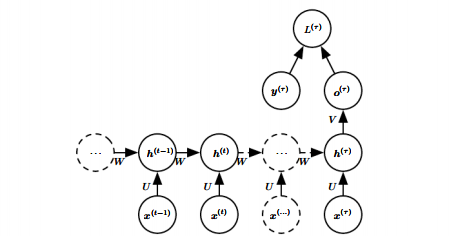
\includegraphics[width=0.9\textwidth]{OFRNN}
				\caption{The structure of RNN(Only One Output)}
			\end{figure}
			\textbf{The update equations for the forward propagation is}
			\begin{flalign*}
			\mathbf{a}^{(t)} &= \mathbf{b} + \mathbf{Wh}^{(t-1)} + \mathbf{Ux}^{(t)} \qquad 1 \leq t \leq \tau\\
			\mathbf{h}^{(t)} &= tanh(\mathbf{a}^{(t)}) \qquad 1 \leq t \leq \tau\\
			\mathbf{O}^{(\tau)} &= \mathbf{c} + \mathbf{Vh}^{(\tau)} \\
			\hat{\mathbf{y}}^{(\tau)} &= softmax(\mathbf{O}^{(\tau)})
			\end{flalign*}
			where the parameters are bias vectors $\mathbf{b}$ and $\mathbf{c}$ along with the weight matrices
			$\mathbf{U}$, $\mathbf{V}$ and $\mathbf{W}$, respectively for input-to-hidden, hidden-to-output and hidden-to- hidden connections
	\end{itemize}

	\subsection{Teaching Force}
		Note that in the second pattern,it lacks hidden-to-hidden
		recurrence.
		\begin{itemize}
			\item It is less powerful.
			\item However,for any loss function based on comparing the prediction at time t to the training target at time t, all the time steps are decoupled.
			\item Training can thus be parallelized, with the gradient for each step t computed in isolation.
		\end{itemize}
		\begin{figure}[H]
			\centering
			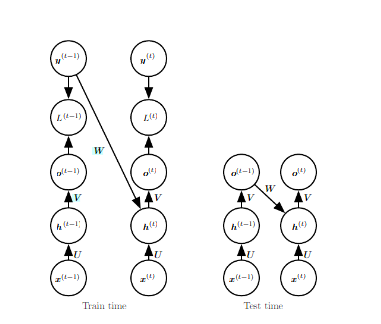
\includegraphics[width=0.9\textwidth]{TF}
			\caption{The representation of Teaching Force}
		\end{figure}
	The parallelization is the concept of \textbf{Teaching Force}.
		\begin{itemize}
			\item Teacher forcing is a procedure that emerges from the maximum likelihood criterion, in which during training the
			model receives \textbf{the ground truth output} $y^{(t)}$ as input at time t + 1.
			\item Take a sequence with two time steps as an example. The conditional maximum likelihood criterion is
			\begin{flalign*}
			log p(\mathbf{y}^{(1)},\mathbf{y}^{(2)}|\mathbf{x}^{(1)},\mathbf{x}^{(2)}) \\
			= log p(\mathbf{y}^{(2)} | \mathbf{y}^{(1)},\mathbf{x}^{(1)},\mathbf{x}^{(2)}) + log p(\mathbf{y}^{(1)} | \mathbf{x}^{(1)},\mathbf{x}^{(2)})
			\end{flalign*}
			\item In this example, we see that at time t = 2, the model is trained to maximize the \textbf{conditional probability} of $\mathbf{y}^{(2)}$ given both the $\mathbf{x}$ sequence so far and the previous $\mathbf{y}$ value from the training.
		\end{itemize}	

	\section{Development of RNN}
	
	\subsection{Encoder-Decoder}
		\begin{figure}[H]
			\centering
			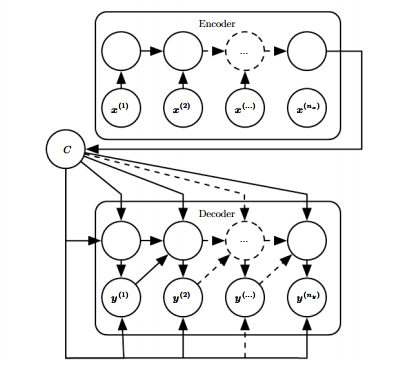
\includegraphics[width=0.9\textwidth]{Encoder-Decoder}
			\caption{The structure of Encoder-Decoder}
		\end{figure}

		\begin{itemize}
			\item It's an RNN that can be trained to map an input sequence to an output sequence which is not necessarily of the same length.
			\item First, we have an \textbf{encoder} or \textbf{input} RNN that processes the input sequence. The encoder emits the context C, usually as a simple function of its final hidden state.
			\item The context C might be a vector or sequence of
			vectors that summarize the input sequence $\mathbf{X} = (\mathbf{x}^{(1)},\ldots,\mathbf{x}^{(n_x)})$.
			\item Then we have a \textbf{decoder} or \textbf{output} RNN that is conditioned on that fixed-length vector $\mathbf{X}$ to generate the output sequence $(\mathbf{y}^{(1)},\ldots,\mathbf{y}^{(n_y)})$.
			\item The two RNNs are trained jointly to maximize the average of \\
			$log P(\mathbf{y}^{(1)},\ldots,\mathbf{y}^{(n_y)}|\mathbf{x}^{(1)},\ldots,\mathbf{x}^{(n_x)})$ over all the pairs of x and y
			sequences in the training set.
		\end{itemize}
	\subsection{Deep RNN}
		The computation in most RNNs can be decomposed into three blocks of parameters and associated transformations:

		\begin{itemize}
			\item[1.] from the input to the hidden state
			\item[2.] from the previous hidden state to the next hidden state
			\item[3.] from the hidden state to the output
		\end{itemize}
		Experimental evidence (Graves et al., 2013; Pascanu et al., 2014a) strongly suggests that we need \textbf{enough depth} in order to perform the required mappings in each of these operations.
		\begin{figure}[H]
			\centering
			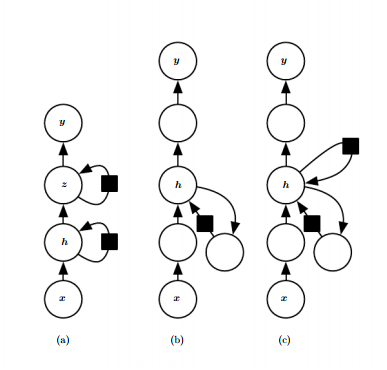
\includegraphics[width=0.9\textwidth]{DeepRNN}
			\caption{Some kind of Structure for Deep RNN}
		\end{figure}
	A recurrent neural network can be made deep in many ways (Pascanu
	et al., 2014a). 
	\begin{itemize}
		\item (a) The hidden recurrent state can be broken down into groups organized hierarchically. 
		\item (b) Deeper computation (e.g., an MLP) can be introduced in the input-to- hidden, hidden-to-hidden and hidden-to-output parts. This may lengthen the shortest path linking different time steps. 
		\item (c) The path-lengthening effect can be mitigated by introducing skip connections.
	\end{itemize}
		
	\subsection{Recursive Neural Network}
		\begin{itemize}
			\item Recursive neural networks represent yet another generalization of recurrent networks, with a different kind of computational graph, which is structured as a \textbf{deep tree}, rather than the chain-like structure of RNNs.
			\item One clear advantage of recursive nets over recurrent nets is that for a sequence of the same length $\tau$, the depth (measured as the number of compositions of nonlinear operations) can be drastically reduced from $\tau$ to $O(log \tau)$.
			\item However,how to \textbf{best structure the tree} is an open question.
		\end{itemize}
		\begin{figure}[H]
			\centering
			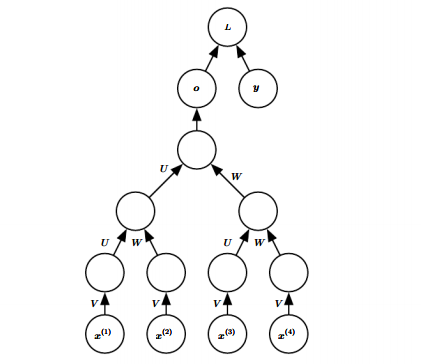
\includegraphics[width=0.9\textwidth]{ReNN}
			\caption{The structure of Recursive Neural Network}
		\end{figure}

\section{The Challenge of long term dependency}
\subsection{Computation of the gradient}
Computing the gradient through a recurrent neural network is straightforward. One simply applies the generalized back-propagation algorithm to the network. \\
What we need to take care of is that the back propagation should be computed through \textbf{the time step}. We will use the example of computing the gradients of Vanilla RNN above to show how the BP algorithm behaves. \\
Denote the final loss as $L$,we can see 
\begin{equation}
\frac{\partial L}{\partial L^{(t)}} = 1  \ ,1\le t \le \tau
\end{equation}
Assume the output function is softmax function and the loss is negative log-likelihood function, The gradient $\nabla_{o^{(t)}}L$ on the outputs at time step t, for all i,t, is as follows:
\begin{equation}
(\nabla_{o^{(t)}}L)_i = \frac{\partial L}{\partial L^{(t)}}\frac{\partial L^{(t)}}{\partial o_i^{(t)}} = \hat{y_i}^{(t)} - 1_{i,y^{(t)}}
\end{equation}
At the final time step $\tau$, we have
\begin{equation}
\nabla_{h^{(\tau)}}L = V^{T}\nabla_{o^{(\tau)}}L
\end{equation}
with 
\begin{eqnarray}
\nabla_{h^{(t)}}L & = & (\frac{\partial h^{(t+1)}}{\partial h^{(t)}})^{T}\nabla_{h^{(t+1)}}L + (\frac{\partial o^{(t)}}{\partial h^{(t)}})^{T}\nabla_{o^{(t)}}L \\
 & = & W^T\nabla_{h^{(t+1)}}L diag(1 - (h^{(t+1)})^2) + V^T\nabla_{o^{(t)}}L
\end{eqnarray}
from $t = \tau -1$ down to $t = 1$. \\
With these, the gradient on the remaining parameters is given by:
\begin{eqnarray}
\nabla_{c}L & = & \sum_{t=1}^{\tau} \nabla_{o^{(t)}}L \\
\nabla_{b}L & = & \sum_{t=1}^{\tau} diag(1 - (h^{(t)})^2)\nabla_{h^{(t)}}L \\
\nabla_{V}L & = & \sum_{t=1}^{\tau}(\nabla_{o^{(t)}}L)h^{(t)^T} \\
\nabla_{W}L & = & \sum_{t=1}^{\tau} diag(1 - (h^{(t)})^2)(\nabla_{h^{(t)}}L)h^{(t-1)^T} \\
\nabla_{U}L & = & \sum_{t=1}^{\tau} diag(1 - (h^{(t)})^2)(\nabla_{h^{(t)}}L)x^{(t)^T}
\end{eqnarray}
\subsection{Challenge of long term dependency}
From the computation above, we can see in the recurrent network, it involves the composition of the same function multiple times, once per time step. Recall the equation:
\begin{equation}
\nabla_{h^{(t)}}L = W^T\nabla_{h^{(t+1)}}L diag(1 - (h^{(t+1)})^2) + V^T\nabla_{o^{(t)}}L
\end{equation}
From the knowledge of linear algebra, we can see the recurrent composition causes eigenvalues with magnitude less than one to decay to zero and eigenvalues with magnitude greater than one to explode.  \\
Let's first focus on the impact of vanishing gradient.Specifically, whenever the model is able to represent long term dependencies, the gradient of a long term interaction has \textbf{exponentially smaller magnitude} than
the gradient of a short term interaction. It does not mean that it is impossible to learn, but that it might take a very long time to learn long-term dependencies, because the signal about these dependencies will tend to be hidden by the smallest fluctuations arising from short-term dependencies. \\
We will discuss various approaches that have been proposed to reduce the difficulty of learning long- term dependencies, but the problem of learning long-term dependencies remains one of the main challenges in deep learning.

\subsection{Long Short Term Memory}
In the LSTM model, we use a forget unit $f_i^{(t)}$,that sets this weight to a value between 0 and 1 via a sigmoid unit:
\begin{equation}
f_i^{(t)} = \sigma(b_i^f + \sum_jU_{i,j}^fx_j^{(t)} + \sum_jW_{i,j}^fh_j^{(t-1)})
\end{equation}
where $x^{(t)}$ is the current input vector and $h^{(t)}$ is the current hidden layer vector, containing the outputs of all the LSTM cells, and $b^f$,$U^f$,$W^f$,are respectively biases, input weights and recurrent weights for the forget gates. \\
 The LSTM cell internal state is thus updated as the following, with a conditional self-loop weight $f_i^{(t)}$
\begin{equation}
s_i^{(t)} = f_i^{(t)} \ast s_i^{(t-1)} + g_i^{(t)} \ast \sigma(b_i + \sum_jU_{i,j}x_j^{(t)} + \sum_jW_{i,j}h_j^{(t-1)})
\end{equation}
where b, U and W respectively denote the biases, input weights and recurrent weights into the LSTM cell and $\ast$ means the multiplication by elements($.\ast$ in MATLAB). \\
The external input gate unit $g_i^{(t)}$ is computed similarly to the forget gate (with a sigmoid unit to obtain a gating value between 0 and 1, but with its own parameters:

\begin{equation}
g_i^{(t)} = \sigma(b_i^g + \sum_jU_{i,j}^gx_j^{(t)} + \sum_jW_{i,j}^gh_j^{(t-1)})
\end{equation}The output $h_i^{(t)}$ of the LSTM cell can also be shut off, via the output gate $o_i^{(t)}$, which also uses a sigmoid unit for gating:

\begin{equation}
h_i^{(t)} = tanh(s_i^{(t)}) \ast o_i^{(t)}
\end{equation}
\begin{equation}
o_i^{(t)} = \sigma(b_i^o + \sum_jU_{i,j}^ox_j^{(t)} + \sum_jW_{i,j}^oh_j^{(t-1)})
\end{equation}
LSTM networks have been shown to learn long-term dependencies more easily than the simple recurrent architectures.
\begin{figure}[H]
	\centering
	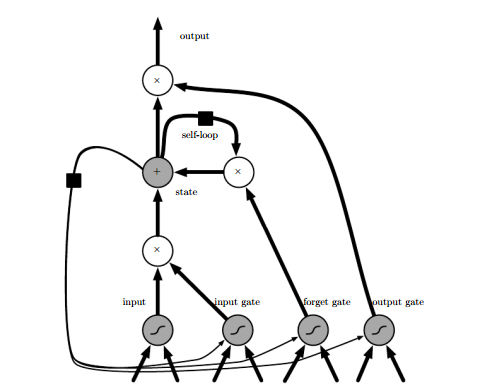
\includegraphics[width=0.9\textwidth]{LSTM}
	\caption{Block diagram of the cell of LSTM recurrent network. Cells are connected recurrently to each other, replacing the usual hidden units of ordinary recurrent networks. An input feature is computed with a regular artificial neuron unit. Its value can be accumulated into the state if the sigmoidal input gate allows it. The state unit has a linear self-loop whose weight is controlled by the forget gate. The output of the cell can be shut off by the output gate. All the gating units have a sigmoid nonlinearity, while the input unit can have any squashing nonlinearity. The state unit can also be used as an extra input to the gating units. The black square indicates a delay of a single time step.}
\end{figure}
From the equations above, we'll give a brief explanation(not strict!) here why the LSTM works for the long-term dependency. We will just focus on the gradient vanishing. \\
First, we have 
\begin{equation}
s_i^{(t)} = f_i^{(t)} \ast s_i^{(t-1)} + g_i^{(t)} \ast \sigma(b_i + \sum_jU_{i,j}x_j^{(t)} + \sum_jW_{i,j}h_j^{(t-1)})
\end{equation}
hence we get
\begin{equation}
\frac{\partial s_i^{(t+k)}}{\partial s_i^{(t)}} \approx \prod_{j=t+1}^{t+k} diag(f_i^{(j)}) + ...
\end{equation}
where the $...$ things are some products which are vanishing to zero as k increases(just like we talked above). If in each time step j($t \le j \le t+k$), $f_i^{(j)} \approx \textbf{1}$(It forgets nothing!),we can see that $\frac{\partial s_i^{(t+k)}}{\partial s_i^{(t)}}$ is almost an identity matrix in the long term, and that means we can connect the information between long time steps together. We can go to the paper <LONG SHORT-TERM MEMORY>(Schmidhuber $\&$ Hochreiter,1997) for the detailed discussion.
\subsection{Other Gated RNNs}
Let's take a look at the recent work on gated RNNs, whose units are also known as gated recurrent units or GRUs (Cho et al., 2014b;Chung et al., 2014, 2015a; Jozefowicz et al., 2015; Chrupala et al., 2015). \\
The main difference with the LSTM is that a single gating unit simultaneously controls the forgetting factor and the decision to update the state unit. The update equations are the following:

\begin{equation}
h_i^{(t)} = u_i^{(t-1)} \ast h_i^{(t-1)} + (1 - u_i^{t-1}) \ast \sigma(b_i + \sum_jU_{i,j}x_j^{(t-1)} + \sum_jW_{i,j}r_j^{(t)}h_j^{(t-1)})
\end{equation}
where $u$ is 'update' gate and $r$ is 'reset' gate. The values are determined by:
\begin{equation}
u_i^{(t)} = \sigma(b_i^u + \sum_jU_{i,j}^ux_j^{(t)} + \sum_jW_{i,j}^uh_j^{(t-1)})
\end{equation}
and
\begin{equation}
r_i^{(t)} = \sigma(b_i^r + \sum_jU_{i,j}^rx_j^{(t)} + \sum_jW_{i,j}^rh_j^{(t-1)})
\end{equation}
\section{Optimization methods for RNN}
\subsection{Clipping gradients}
As discussed before, strongly nonlinear functions such as those computed by a recurrent net over many time steps tend to have derivatives that can be either very large or very small in magnitude. \\
The difficulty that arises is that when the parameter gradient is very large, a gradient descent parameter update could throw the parameters very far, into a region where the objective function is larger, undoing much of the work before.The gradient tells us the direction that corresponds to the steepest descent within an infinitesimal region surrounding the current parameters. \\
A simple type of solution has been in use by practitioners for many years:
clipping the gradient. One step is to clip the norm $||g||$ of the gradient g (Pascanu et al., 2013) just before the parameter update:
\begin{eqnarray}
\text{if} \ & ||g||  > v \\
& g\leftarrow \frac{g v}{||g||}
\end{eqnarray}
Because the gradient of all the parameters (including different groups of parameters, such as weights and biases) is renormalized jointly with a single scaling factor, the method has the advantage that it guarantees that each step is \textbf{still in the gradient direction}. Although the parameter updating has the same direction as the true gradient, with gradient norm clipping, the parameter update vector norm is now bounded. This bounded gradient avoids performing a detrimental step when the gradient explodes.
\begin{figure}[H]
	\centering
	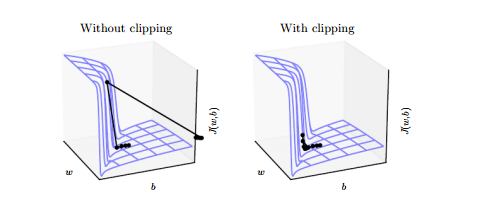
\includegraphics[width=0.9\textwidth]{Clipgrad}
	\caption{Example of the effect of gradient clipping in a recurrent network with two parameters w and b. Gradient clipping can make gradient descent perform more reasonably in the vicinity of extremely steep cliffs. These steep cliffs commonly occur in recurrent networks near where a recurrent network behaves approximately linearly. The cliff is exponentially steep in the number of time steps because the weight matrix is multiplied by itself once for each time step. (Left)Gradient descent without gradient clipping overshoots the bottom of this small ravine, then receives a very large gradient from the cliff face. The large gradient catastrophically propels the parameters outside the axes of the plot. (Right)Gradient descent with gradient clipping has a more moderate reaction to the cliff. While it does ascend the cliff face, the step size is restricted so that it cannot be propelled away from steep region near the solution. Figure adapted with permission from Pascanu et al. (2013).
}
\end{figure}
\subsection{Regularizing to Encourage Information Flow}
Gradient clipping helps to deal with exploding gradients, but it does not help with vanishing gradients.To address vanishing gradients and better capture long-term dependencies, an idea is to regularize or constrain the parameters so as to encourage 'information flow'. \\
In particular, we would like the gradient vector $\nabla_{h^{(t)}}L$ being back-propagated to maintain its magnitude, even if the loss function only penalizes the output at the end of the sequence. Formally, we want
\begin{equation}
(\nabla_{h^{(t)}}L) \frac{\partial h^{(t)}}{\partial h^{(t-1)}}
\end{equation}
to be as large as 
\begin{equation}
\nabla_{h^{(t)}}L
\end{equation}
With this objective, Pascanu et al. (2013) propose the following regularizer:
\begin{equation}
\Omega = \sum_{t}(\frac{|(\nabla_{h^{(t)}}L) \frac{\partial h^{(t)}}{\partial h^{(t-1)}}|}{|\nabla_{h^{(t)}}L|} - 1)^2
\end{equation}
The experiments with this regularizer suggest that, if combined with the norm clipping, the regularizer can considerably increase the span of the dependencies that an RNN can learn.
